\documentclass{tudelft-report}
\usepackage{natbib}
% Start of 'ignore natbib' hack
\let\bibhang\relax
\let\citename\relax
\let\bibfont\relax
\let\Citeauthor\relax
\expandafter\let\csname ver@natbib.sty\endcsname\relax
\usepackage{changes}
\usepackage{subcaption}
\usepackage[export]{adjustbox}
\usepackage{float}
\restylefloat{table}
\usepackage[style=authoryear,sorting=nyt,backend=biber]{biblatex}\usepackage{csquotes}
\usepackage{hyperref}
\usepackage[inline]{enumitem}
\usepackage{xcolor}
\usepackage{listings}
\graphicspath{ {figures/} }
\addbibresource{report.bib}
\begin{document}
\frontmatter
\title[tudelft-white]{\fontsize{30}{5}\fontshape{sl}\selectfont Implementing a Sensor Observation Service for Wi-Fi tracking data}
\subtitle[tudelft-white]{\fontsize{20}{1.2}\selectfont A case study of TU Delft Campus}
\author[tudelft-white]{\fontsize{15}{10}\selectfont Balazs Dukai
\vskip 0.15cm Matthijs Bon
\vskip 0.15cm Xander den Duijn}
\affiliation{Technische Universiteit Delft}
\coverimage{cover_article.jpg}
\setpagecolor{tudelft-cyan}
\makecover[split]
%% Include an optional title page.
\begin{titlepage}


\begin{center}

%% Insert the TU Delft logo at the bottom of the page.

%% Print the title in cyan.
{\makeatletter
\largetitlestyle\fontsize{64}{94}\selectfont\@title
%\largetitlestyle\color{tudelft-cyan}\Huge\@title
\makeatother}

%% Print the optional subtitle in black.
{\makeatletter
\ifx\@subtitle\undefined\else
    \bigskip
   {\tudsffamily\fontsize{22}{32}\selectfont\@subtitle}    
    %\titlefont\titleshape\LARGE\@subtitle
\fi
\makeatother}

\bigskip
\bigskip

by
%door

\bigskip
\bigskip

%% Print the name of the author.
{\makeatletter
%\largetitlefont\Large\bfseries\@author
\largetitlestyle\fontsize{26}{26}\selectfont\@author
\makeatother}

\bigskip
\bigskip

{\fontsize{15}{0.2}\selectfont GEO1007 course during the MSc programme Geomatics for the built environment
%ter verkrijging van de graad van Master of Science

at the Delft University of Technology,}
%aan de Technische Universiteit Delft,

\vfill

\begin{tabular}{lll}
    Project duration: & \multicolumn{2}{l}{April 16, 2016 -- June 9, 2016} \\
\end{tabular}
%% Only include the following lines if confidentiality is applicable.

\bigskip
\bigskip
\bigskip
\bigskip
%\\[1cm]
to be presented on Friday May 20, 2016.
\end{center}

\begin{tikzpicture}[remember picture, overlay]
    \node at (current page.south)[anchor=south,inner sep=0pt]{
        
\includegraphics{cover/logo_black}
    };
\end{tikzpicture}

\end{titlepage}

	

\chapter*{Preface}
\setheader{Preface}

Preface\ldots

\begin{flushright}
{\makeatletter\itshape
    \@author \\
    Delft, January 2013
\makeatother}
\end{flushright}



\tableofcontents

%% Use Arabic numerals for the page numbers of the chapters.
\mainmatter
%\input{chapter-0}
\chapter{Introduction}
% General introduction, scope of the project
This report describes the process and results of the assignment for the GEO1007 course in the MSc Geomatics programme. For this assignment, the authors chose one of seven topics. The chosen topic focusses on implementing a Sensor Observation Service to publish the tracking data derived from the geomatics synthesis project on a server and test it in a SOS client, such as the 52 North application. \\\\
A Sensor Observation Service (SOS) is a service standardized by the Open Geospatial Consortium (OGC). The standard defines a web service interface for the discovery and retrieval of real time or archived data produced by all kinds of sensors like mobile or stationary as well as in-situ or remote sensors (OGC, 2016). A sensor can measure multiple things, e.g. a meteorological sensor can observe properties such as temperature, wind speed, humidity. The SOS standard focusses mainly on the observations of these sensors. \\
In this project, the focus lies on the Wi-Fi network of the TU Delft campus. The wireless access points (AP) used in the Wi-Fi network can be seen as sensors, and the devices registered by the APs can be seen as the measurement. Each devices can be identified by its unique mac address, but also other properties can be measured, i.e. the received signal strength and the signal to noise ratio (SNR). These are all observations that can be retrieved using a SOS. In the next sections the research question, objectives, methods and tools will be discussed.

\section{Problem description}
% What are we going to research, what are we going to build/develop?
%%% Include literature here? That there hasnt been any implementation of SOS for wifi tracking data untill now? %%%
% The difference between SOS for “occupancy” or SOS for “movement”

During this project, the research will be guided by the following question:\\
\textit{How can the 52North webapplication be used to publish and visualize the WiFi tracking data from the TU Delft eduroam network?}\\

This research question can be divided into the following subjects which need to be addressed:
\begin{itemize}
\item Research the 52North database model for a SOS
\item Setting up the SOS server
\item Testing the SOS client
\end{itemize}

These questions can be answerd once the goals and objectives have been established.

\section{Objectives}
% What is the purpose of the research (what will it solve), what is the purpose of the developed app (what can a user do with it)?
% Must, Should, Could, Won't
To answer the research question and subquestions, the purpose of the research has to be clearly defined. The purpose of the research is captured into two main objectives:
\begin{itemize}
\item To provide a method for publishing WiFi-based tracking data through an SOS service and visualize the data in a client. The user can view and subset the data in the client and eventually download it. This allows a quick, preliminary data filtering which speeds up the data analysis workflow.
\item To set up a SES service which pushes newly added tracking data to the client/user.
\end{itemize}
To dive deeper into the steps that need to be taken to answer the research question, the objectives can be divided into sub-goals:\\
\begin{itemize}
\item Automatically transform the raw WiFi-logs from the PostgreSQL database to an SOS-compliant data model.
\item Functionality to download raw WiFi-logs or trajectories.
\item Time series tracking data (subset WiFi-logs with time range) in the client
\end{itemize}
Finally, to structure the objectives and goals and to define the scope of the project, the objectives are grouped using the MoSCoW rules (see \autoref{table:moscow}). To achieve these goals, implementation of the SOS Core Profile is necessary, comprising the mandatory operations: GetCapabilities, DescribeSensor, GetObservation.\\
\begin{table}[]
\centering
\begin{tabular}{@{}llll@{}}
\toprule
\textbf{MUST}                                                                                                                                        & \textbf{SHOULD}                                                                                                                                                         \\ \midrule
\begin{tabular}[c]{@{}l@{}}Automatically transform the raw WiFi-logs \\ from the PostgreSQL database to an SOS-\\ compliant data model.\end{tabular} & \begin{tabular}[c]{@{}l@{}}Functionality to download raw WiFi-logs or \\ trajectories.\end{tabular}                                                                     \\
                                                                                                                                                     &                                                                                                                                                                         \\
\begin{tabular}[c]{@{}l@{}}Time series tracking data (subset WiFi-logs \\ with time range) in the client\end{tabular}                                &                                                                                                                                                                         \\ \midrule
\textbf{COULD}                                                                                                                                       & \textbf{WONT}                                                                                                                                                           \\ \midrule
                                                                                                                                                     & \begin{tabular}[c]{@{}l@{}}Push notification to the user when new data \\ is available\end{tabular}                                                                     \\
                                                                                                                                                     &                                                                                                                                                                         \\
                                                                                                                                                     & \begin{tabular}[c]{@{}l@{}}Push new data to the user. When subscribing, \\ the user can decide to either receive the raw \\ WiFi-logs or the trajectories.\end{tabular}
\caption{MoSCoW Rules}
\label{table:moscow}
\end{tabular}
\end{table}

\section{Methods}
% What methods do we use to get to the objectives?


\subsection{Tools}
% The tools we used, e.g. SQL / PostgreSQL, Python, 52N application
\chapter{Functionality}
% General introduction, what will the chapter discuss?

\section{52North application}
% General introduction of the 52N application, what can it do, implementation, services

\subsection{Database model}
% The database model, why did we chose non-transactional and other choices / assumptions we made 

\subsection{Standards}
% Not sure if needed..


\chapter{Introduction}

\chapter{Status of the application}

% geoserver running
% database working
% able to do queries (getcapabilities, getfeatureofinterest)
% unable to query the actual data
% kvp works, JSON doesn't

The application that was created during the course of this project is almost finished. The steps that needed to be taken to get from the raw Wi-Fi data to the SOS on the geoserver have all been taken, but some debugging is still to be done to have a final working application. \\
Setting up the geoserver was the easy part. The webapp that 52°North provided could be imported directly into the geoserver running on the local machines. The configuration of the 52°North SOS was slightly harder. The original Wi-Fi tracking data is on a remote server on the TU Delft campus, but the encoding for that server is in 'LATIN1', which is unsupported by the 52°North SOS. It required a new database with new encoding to get the SOS tables in the database. Filling the tables with the tracking data took most of the time, but using the 52°North application as a guide ensured that the correct attributes were used in the tables. \\
Finally, the 52°North webapp could be used to do sample queries on the database to check if the database model was correct. This worked and showed that the database model was correct. \autoref{figure:testqueries} shows such a sample query and the result from the database. 
\begin{figure}[H]
\centering
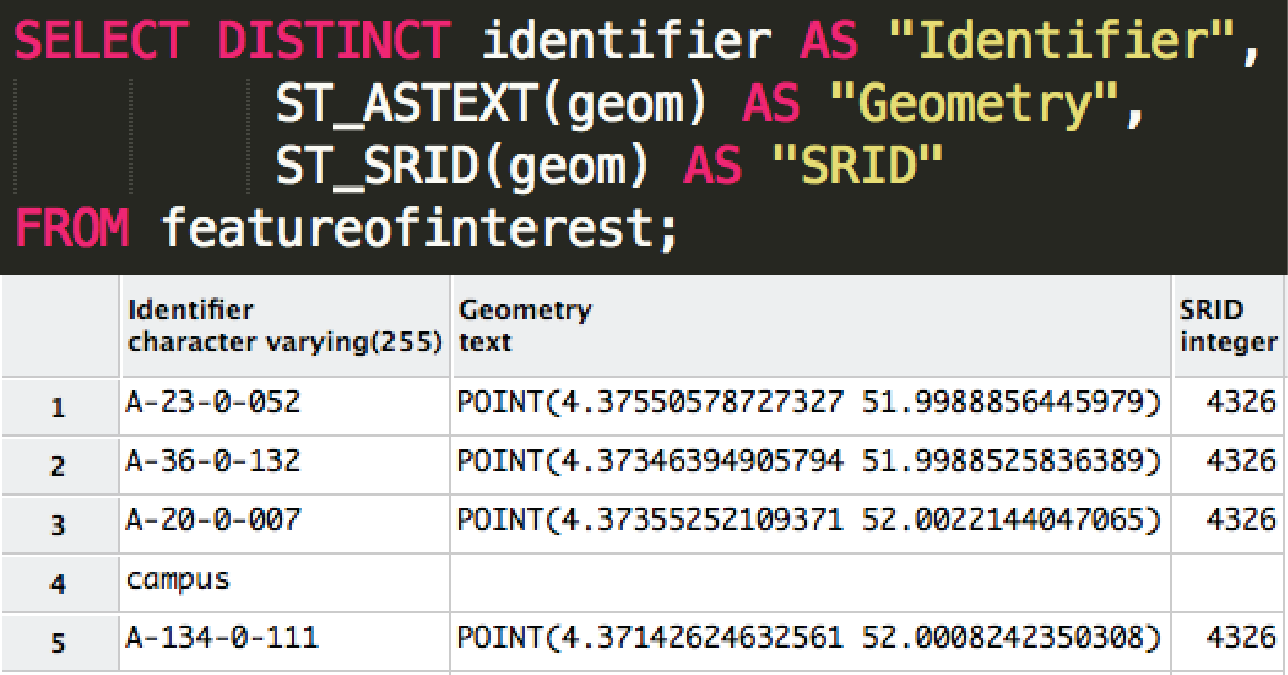
\includegraphics[scale=0.8]{testqueries.png}
\captionsetup{justification=centering}
\caption{Test queries on the database}
\label{figure:testqueries}
\end{figure}

Additionally, sample requests can also be sent. These sample requests can be generated by the 52°North webapp test client. Such requests are GetCapabilities, GetFeatureOfInterest

%% Use letters for the chapter numbers of the appendices.
%%\appendix

%\input{appendix-a}
\nocite{*}
\printbibliography

\end{document}

